\def\duedate{September 14, 2023}
\def\HWnum{2}
\documentclass[10pt,a4paper]{book}

% custom section formatting
\usepackage{titlesec}
\titleformat{\chapter}[display]
{\normalfont\Large\filcenter\sffamily}
{\titlerule[1pt]%
\vspace{1pt}%
\titlerule
\vspace{1pc}%
\LARGE\MakeUppercase{\chaptertitlename} \thechapter}
{1pc}
{\titlerule
\vspace{1pc}%
\Huge}

% appendix handling
\usepackage[toc,page]{appendix}
    
% encoding for file and font
\usepackage[utf8]{inputenc}
\usepackage[T1]{fontenc}

% math formatting/tools
\usepackage{amsmath}
\usepackage{amssymb}
\usepackage{mathtools}
\usepackage[arrowdel]{physics}

% unit formatting
\usepackage{siunitx}
\AtBeginDocument{\RenewCommandCopy\qty\SI}

% figure formatting/tools
\usepackage{graphicx}
\usepackage{float}
\usepackage{subcaption}
\usepackage{multirow}
\usepackage{import}
\usepackage{pdfpages}
\usepackage{transparent}
\usepackage{currfile}

\NewDocumentCommand\incfig{O{1} m}{
    \def\svgwidth{#1\textwidth}
    \import{./Figures/\currfiledir}{#2.pdf_tex}
}

\newcommand{\bef}{\begin{figure}[h!tb]\centering}
\newcommand{\eef}{\end{figure}}

\newcommand{\bet}{\begin{table}[h!tb]\centering}
\newcommand{\eet}{\end{table}}

% hyperlink references 
\usepackage{hyperref}
\hypersetup{
    colorlinks=true,
    linkcolor=blue,
    filecolor=magenta,
    urlcolor=cyan,
    pdftitle={Physics 1 Notes},
    pdfauthor={Richard Whitehill},
    pdfpagemode=FullScreen
}
\urlstyle{same}

\newcommand{\eref}[1]{Eq.~(\ref{eq:#1})}
\newcommand{\erefs}[2]{Eqs.~(\ref{eq:#1})--(\ref{eq:#2})}

\newcommand{\fref}[1]{Fig.~(\ref{fig:#1})}
\newcommand{\frefs}[2]{Fig.~(\ref{fig:#1})--(\ref{fig:#2})}

\newcommand{\aref}[1]{Appendix~(\ref{app:#1})}
\newcommand{\sref}[1]{Section~(\ref{sec:#1})}
\newcommand{\srefs}[2]{Sections~(\ref{sec:#1})-(\ref{sec:#2})}

\newcommand{\tref}[1]{Table~(\ref{tab:#1})}
\newcommand{\trefs}[2]{Table~(\ref{tab:#1})--(\ref{tab:#2})}

% tcolorbox formatting/definitions
\usepackage[most]{tcolorbox}
\usepackage{xcolor}
\usepackage{xifthen}
\usepackage{parskip}

\definecolor{peach}{rgb}{1.0,0.8,0.64}

\DeclareTColorBox[auto counter, number within=chapter]{defbox}{O{}}{
    enhanced,
    boxrule=0pt,
    frame hidden,
    borderline west={4pt}{0pt}{green!50!black},
    colback=green!5,
    before upper=\textbf{Definition \thetcbcounter \ifthenelse{\isempty{#1}}{}{: #1} \\ },
    sharp corners
}

\newcommand*{\eqbox}{\tcboxmath[
    enhanced,
    colback=black!10!white,
    colframe=black,
    sharp corners,
    size=fbox,
    boxsep=8pt,
    boxrule=1pt
]}

\newtcolorbox[auto counter, number within=chapter]{exbox}{
    parbox=false,
    breakable,
    enhanced,
    sharp corners,
    boxrule=1pt,
    colback=white,
    colframe=black,
    before upper= \textbf{Example \thetcbcounter:}\,,
    before lower= \textbf{Solution:}\,,
    segmentation hidden
}

\newtcolorbox{resbox}{
    enhanced,
    colback=black!10!white,
    colframe=black,
    boxrule=1pt,
    boxsep=0pt,
    top=2pt,
    ams nodisplayskip,
    sharp corners
}


\begin{document}

\prob{1}{

Using Gauss' theorem we found that, in cylindrical coordinates $(\rho, \phi,z)$, the electric field of an infinitely long, thin rod carrying charge $\lambda$ per unit length is given by
\begin{eqnarray}
    \va*{E}(\rho) = \frac{\lambda}{2 \pi \epsilon_{0}} \frac{\vu*{e}_{\rho}}{\rho}
.\end{eqnarray}
Obtain this result by a direct integration using the formula
\begin{eqnarray}
    \label{eq:direct-E}
    \va*{E}(\va*{r}) = \frac{1}{4 \pi \epsilon_0} \int_{V} \rho(\va*{r}') \frac{\va*{r} - \va*{r}'}{|\va*{r} - \va*{r}'|^3} \dd{V'}
.\end{eqnarray}
Similarly, using 
\begin{eqnarray}
    \label{eq:potential-int}
    \Phi(\va*{r}) = \frac{1}{4\pi\epsilon_0} \int_{V} \frac{\rho(\va*{r}')}{|\va*{r} - \va*{r}'|} \dd{V'}
,\end{eqnarray}
find the electric potential corresponding to this field.
Show that $\Phi(\va*{r}) \equiv \Phi(\rho,\phi,z)$ depends in this case on $\rho$ only, and assume that $\Phi(\rho = \rho_0) = 0$ to fix additive constant.

}

\sol{

Consider an infinitely long and thin rod (with charge per unit length $\lambda$) lying along the $z$-axis.
Notice then that the charge density for this rod is given as $\rho(\va*{r}) = \lambda \delta(x)\delta(y)$.
The electric field of this configuration is then found to as
\begin{eqnarray}
    \begin{aligned}
        \va*{E}(\va*{r}) &= \frac{1}{4 \pi \epsilon_0} \int_{V} \lambda \delta(x') \delta(y') \frac{\va*{r} - \va*{r}'}{| \va*{r} - \va*{r}' |^3} \dd{x'} \dd{y'} \dd{z'} \\
                         &= \frac{\lambda}{4 \pi \epsilon_0} \int_{-\infty}^{\infty} \frac{x \vu*{e}_{x} + y \vu*{e}_{y} + (z - z') \vu*{e}_{z}}{[x^2 + y^2 + (z - z')^2]^{3/2}} \dd{z'}
    \end{aligned}
.\end{eqnarray}
Observe that we can switch to cylindrical coordinates, giving
\begin{eqnarray}
    \va*{E}(\va*{r}) = \frac{\lambda}{4 \pi \epsilon_0} \Bigg[ \vu*{e}_{\rho} \int_{-\infty}^{\infty}  \frac{\rho}{[\rho^2 + (z - z')^2]^{3/2}} \dd{z'} + \vu*{e}_{z} \int_{-\infty}^{\infty} \frac{z - z'}{[\rho^2 + (z - z')^2]^{3/2}} \dd{z'} \Bigg]
.\end{eqnarray}
Observe that the second integral is zero by symmetry since the integrand is odd in $z - z'$.
Thus,
\begin{eqnarray}
    \eqbox{
    \va*{E}(\va*{r}) = \frac{\lambda}{4 \pi \epsilon_0 \rho^2} \vu*{e}_{\rho} \int_{\pi/2}^{-\pi/2} \frac{1}{\sec^3{\theta}} (-\rho \sec^2{\theta}) \dd{\theta} = \frac{\lambda}{2 \pi \epsilon_0 \rho} \vu*{e}_{\rho} \int_{0}^{\pi/2} \cos{\theta} \dd{\theta} = \frac{\lambda}{2 \pi \epsilon_0 \rho} \vu*{e}_{\rho}
}
,\end{eqnarray}
where we have used the replacement $z - z' = \rho \tan{\theta}$.

Similarly, we can find the electric potential
\begin{eqnarray}
    \begin{aligned}
        \Phi(\va*{r}) &= \frac{1}{4 \pi \epsilon_0} \int \frac{\lambda \delta(x') \delta(y')}{\sqrt{(x - x')^2 + (y - y')^2 + (z - z')^2}} \dd{x'} \dd{y'} \dd{z'} = \frac{1}{4 \pi \epsilon_0} \\
                      &= \frac{\lambda}{4 \pi \epsilon_0} \int_{-\infty}^{\infty} \frac{1}{\sqrt{\rho^2 + (z - z')^2}} \dd{z'} \\
                      &= \frac{\lambda}{4 \pi \epsilon_0} \int_{-\pi/2}^{\pi/2} \sec{\theta} \dd{\theta}
    .\end{aligned}
\end{eqnarray}
We run into some trouble here, however.
Recall that \eref{potential-int} assumes that we place ground at $r \rightarrow \infty$, but our charge distribution stretches to $z \rightarrow \infty$.
To remedy this situation, we will redefine ground to remove the infinity as follows.
First, we will consider a finite line charge of length $2a$ centered at the origin, recovering the infinite line charge by taking $a \rightarrow \infty$ after some manipulations.
Doing so, we find
\begin{eqnarray}
    \begin{aligned}
        \Phi(\rho) &= \frac{\lambda}{4 \pi \epsilon_0} \int_{-\theta(a)}^{\theta(a)} \sec{\theta} \dd{\theta} = \frac{\lambda}{2 \pi \epsilon_0 \rho} \ln{(\tan{\theta} + \sec{\theta})} \Big|_{0}^{\arctan{a/\rho}} \\
        &= \frac{\lambda}{4 \pi \epsilon_0} \ln{\Big( \tan{\theta} + \sqrt{1 + \tan^2{\theta}} \Big)} \Big|_{-\arctan{a/\rho}}^{\arctan{a/\rho}} \\
        &= \frac{\lambda}{4 \pi \epsilon_0} \ln( \frac{a + \sqrt{ \rho^2 + a^2 }}{-a + \sqrt{\rho^2 + a^2}} ) = \frac{\lambda}{4 \pi \epsilon_0} \ln\Bigg[ \frac{1 + \sqrt{1 + ( \rho/a )^2}}{-1 + \sqrt{1 + ( \rho/a )^2}} \Bigg]
    .\end{aligned}
\end{eqnarray}
The problem with our original integration is now manifestly obvious.
In the limit $a \rightarrow \infty$ the potential is logarithmically divergent since the denominator of the argument goes to zero.
As it stands, the potential is defined as $\Phi(\rho) - \Phi_{\infty}$, where $\Phi_{\infty} \rightarrow \infty$.
We now shift the ground of our potential to $\rho = \rho_0$ such that $\Phi(\rho_0) = 0$\footnote{This is where the magic is: $\Phi \rightarrow [ \Phi(\rho) - \Phi_{\infty}] - [\Phi(\rho_{0}) - \Phi_{\infty}]$. It is clear then that the $\Phi_{\infty}$ contribution (which is infinite) cancels out.}
\begin{eqnarray}
    \Phi(\rho) \rightarrow \Phi(\rho) - \Phi(\rho_0) = \frac{\lambda}{4 \pi \epsilon_0} \ln{ \Bigg[ \Bigg( \frac{1 + \sqrt{1 + (\rho/a)^2}}{-1 + \sqrt{1 + (\rho/a)^2}} \Bigg) \Bigg( \frac{-1 + \sqrt{1 + (\rho_0/a)^2}}{1 + \sqrt{1 + (\rho_0/a)^2}} \Bigg) \Bigg] }
.\end{eqnarray}
Now we can take the limit $a \rightarrow \infty$, expanding in $\rho/a$ and neglecting standalone higher order terms:
\begin{eqnarray}
    \eqbox{ \Phi(\rho) = \frac{\lambda}{4 \pi \epsilon_0} \ln{ \Bigg[ \frac{2}{\frac{1}{2} (\rho/a)^2} \frac{\frac{1}{2} (\rho_0/a)^2}{2} \Bigg] } = \frac{\lambda}{2 \pi \epsilon_0} \ln( \frac{\rho_0}{\rho} ) }
,\end{eqnarray}
which is finite for $\rho > 0$ and has $\Phi(\rho_0) = 0$ as desired.

}


\prob{2}{

    Each of three charged spheres of radius $a$, one conducting, one having a uniform charge density within its volume, and one having a spherically symmetric charge density that varies radially as $r^{n}~(n > -3)$, has a total charge $Q$.
Use Gauss' theorem to obtain the electric fields both inside and outside each sphere.
Sketch the behavior of the fields as a function of radius for the first two spheres, and for the third with $n = \pm 2$.

}

\sol{

Gauss' theorem states $\int \va*{E} \cdot \dd{\va*{S}} = Q/\epsilon_0$.
Note that outside these spheres ($r \ge a$), where the charge density is zero, Gauss' law always gives the same answer
\begin{eqnarray}
   \va*{E} = \frac{Q}{4 \pi \epsilon_0 r^2} \vu*{e}_{r}
.\end{eqnarray}
Hence, we only need to consider $r < a$ on a case-by-case basis.

For the conducting sphere $\rho = (Q/4 \pi a^2) \delta(r - a)$, implying that 
\begin{eqnarray}
    \eqbox{ E_r = 0 }
,\end{eqnarray}
inside the sphere.

Next, we consider the sphere with uniform charge density $\rho(\va*{r}) = \rho_0 = 3Q/(4 \pi a^3)$ for $r < a$.
In this case, Gauss' law gives
\begin{eqnarray}
    \eqbox{
    E_{r} = \frac{1}{4 \pi \epsilon_0 r^2} \Big( \frac{4}{3} \pi \rho_0 r^3 \Big) = \frac{\rho_0}{3\epsilon_0} r
}
,\end{eqnarray}
inside the sphere.

Finally, we consider the case where the sphere has charge density $\rho(\va*{r}) = \rho_0 r^{n}$, where $\rho_0 = (n+3)Q/(4 \pi a^{n+3})$ such that $\int \rho(\va*{r}) \dd[3]{\va*{r}} = Q$.
Thus, we find
\begin{eqnarray}
    \eqbox{ E = \frac{1}{4 \pi \epsilon_0 r^2} \frac{4 \pi \rho_0 r^{n+3}}{n+3} = \frac{\rho_0}{(n+3) \epsilon_0} r^{n+1} }
.\end{eqnarray}

A plot of the electric fields (normalized to some overall constants) for each setup is shown in Fig. (\ref{fig:prob2}):
\begin{figure}[h!]
    \centering
    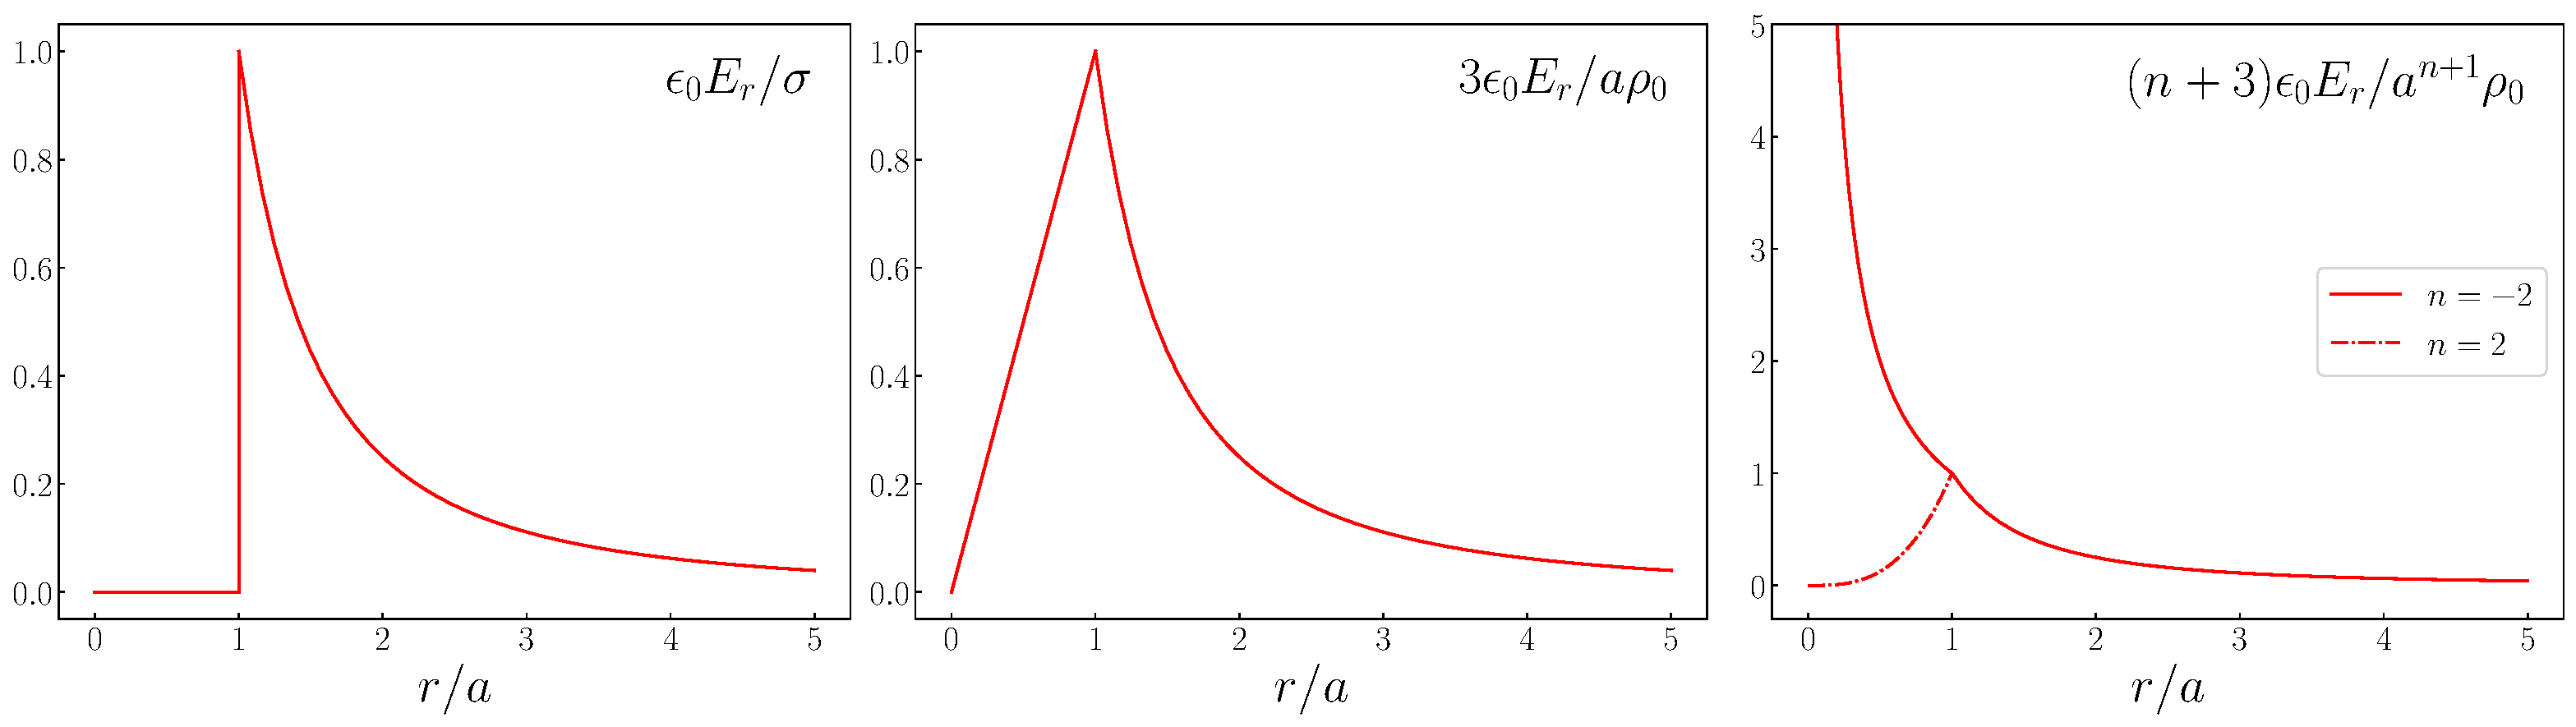
\includegraphics[width=\textwidth]{prob2.pdf}
    \caption{Electric fields for spheres of radius $a$ with \textbf{(Left)} uniform surface charge density, \textbf{(Center)} constant charge density, and \textbf{(Right)} radial power law charge density. Note that in the right-most plot, the dotted and dashed lines are overlapping outside the sphere (i.e. for $r > a$) as expected since the electric field only depends on the total charge enclosed $Q$, which is the same in both cases.}
    \label{fig:prob2}
\end{figure}

}

\newpage

\prob{3}{

The time-averaged potential of a neutral hydrogen atom is given by
\begin{eqnarray}
   \Phi = \frac{q}{4 \pi \epsilon_0} \frac{e^{-\alpha r}}{r} \Big( 1 + \frac{\alpha r}{2} \Big)
,\end{eqnarray}
where $q$ is the magnitude of the electronic charge, and $\alpha^{-1} = a_0/2$, $a_0$ being the Bohr radius.
Find the distribution of charge (both continuous and discrete) that will give this potential and interpret your result physically.

}

\sol{

We can solve this problem by using Poisson's equation $\laplacian{\Phi} = -\rho/\epsilon_0$, which gives
\begin{eqnarray}
    \begin{aligned}
        \rho &= -\frac{q}{4 \pi} \laplacian \frac{e^{-\alpha r}}{r} \Big( 1 + \frac{\alpha r}{r} \Big) = -\frac{q}{4 \pi} \frac{1}{r^2} \pdv{r} \Big[ r^2 \pdv{r} \Big( \frac{e^{-\alpha r}}{r} \Big(1 + \frac{\alpha r}{2} \Big) \Big) \Big] \\
        &= \frac{-q \alpha^3}{8 \pi} e^{-\alpha r} = -\frac{q}{\pi a_0^3} e^{-2r/a_0}
    \end{aligned}
\end{eqnarray}
for $r \ne 0$.
Note that in the midst of all the algebra to arrive at this answer, some factors of $r$ between the numerator and denominator were canceled, which is not quite kosher when $r = 0$.
In this case, we can determine the contribution to $\rho$ from $r = 0$ noting that the hydrogen atom is neutral overall.
Observe that
\begin{eqnarray}
    \int \rho_{r \ne 0}(\va*{r}) \dd[3]{\va*{r}} = -q
.\end{eqnarray}
The only way to cancel this contribution in a way that contributes to the total charge density at $\va*{r} = 0$ (but nowhere else) is via a delta function such that
\begin{eqnarray}
    \eqbox{ \rho(\va*{r}) = q \delta(\va*{r}) - \frac{q}{\pi a_0^3} e^{-2r/a_0} }
,\end{eqnarray}
which clearly gives the correct neutrality of the hydrogen atom: $\int \rho(\va*{r}) \dd[3]{\va*{r}} = 0$.

From this charge density, it is clear that the center or nucleus of the hydrogen atom is a point-like\footnote{at least relative to the scale of the atom} positively charged particle -- the proton.
Furthermore, the second term tells us that the negative part of the hydrogen atom is like a cloud of charge, not localized to any particular position $\va*{r}$.
This is in agreement with the probabilistic nature of the electron's position, given by the wave function $\psi$ and related to its charge density as $\rho_{e} = -q |\psi|^2$.

}


\prob{4}{

A simple capacitor is a device formed by two insulated conductors adjacent to each other.
If equal and opposite charges are placed on the conductors, there will be a certain difference of potential between them.
The ratio of the magnitude of the charge on one conductor to the magnitude of the potential difference is called the capacitance (in SI units it is measured in farads).
Using Gauss' law, calculate the capacitance of \\[3pt]

(a) two large, flat, conducting sheets of area $A$, separated by a small distance $d$; \\[3pt]

(b) two concentric conducting spheres with radii $a,b$ ($b > a$); \\[3pt]

(c) two concentric conducting cylinders of length $L$, large compared to their radii $a,b$ ($b > a$).

}

\begin{figure}[h!]
    \centering
    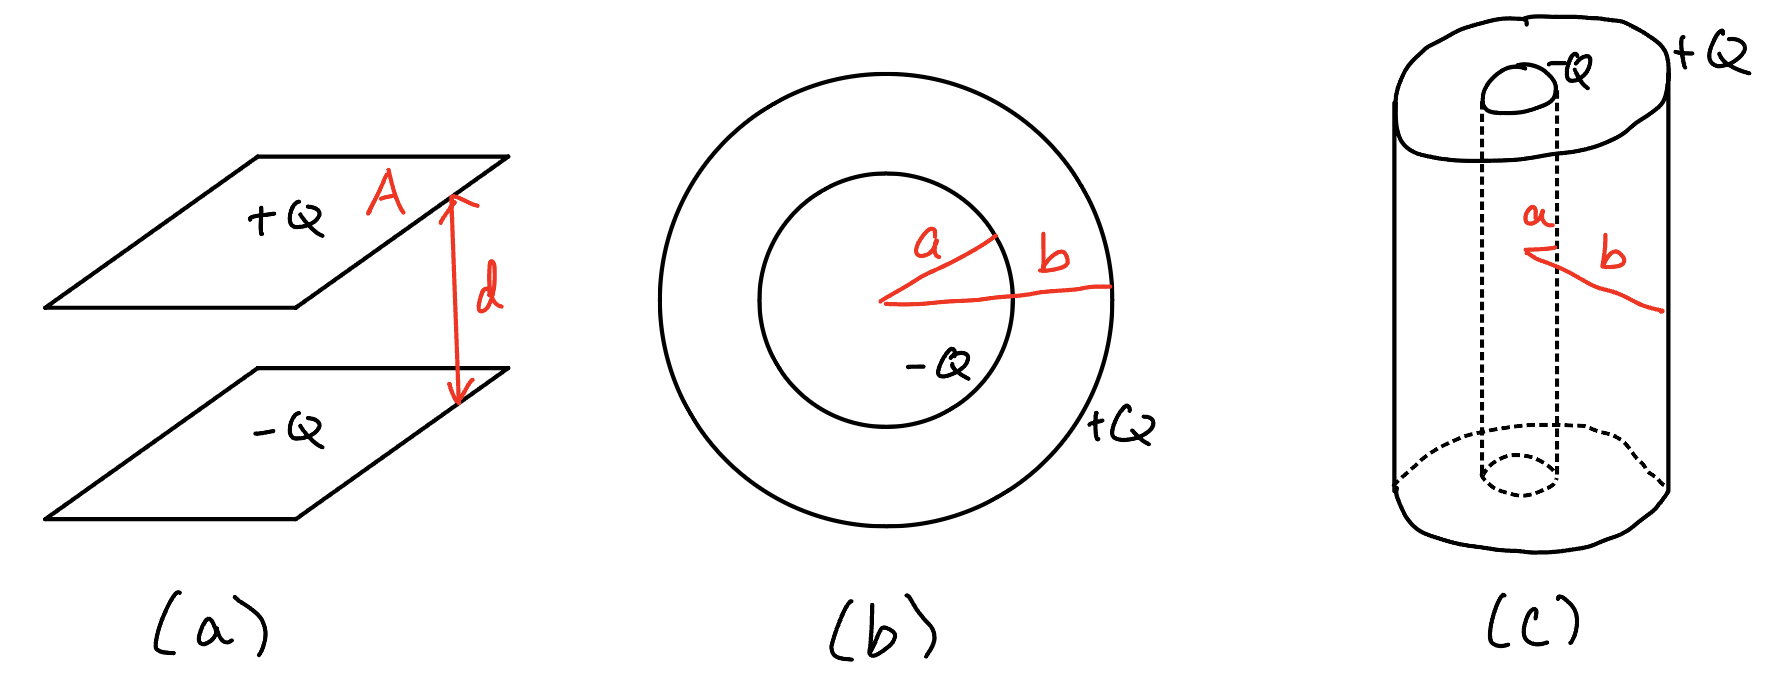
\includegraphics[width=0.8\textwidth]{prob4.jpeg}
    \caption{Sketches of an \textbf{(a)} parallel plate capacitor, \textbf{(b)} spherical capacitor, and \textbf{(c)} cylindrical capacitor.}
    \label{fig:prob4}
\end{figure}

\sol{

(a) The electric field on one side of an infinite plate with surface charge density $\sigma$ is given by
\begin{eqnarray}
    \va*{E} = \frac{\sigma}{2 \epsilon_0} \vu*{n}
,\end{eqnarray}
as found from Gauss' law by taking a small pillbox stradling the plane.
For a finite plane where $d \ll A$, the electric field near the center is approximately the same as that for the infinite plane where $\sigma = Q/A$.
Taking the top and bottom sheets to have charge $+Q$ and $-Q$, respectively, and orienting the $z$-axis to point from the bottom to the top sheet, the total electric field between the plates is
\begin{eqnarray}
    \va*{E} = \va*{E}_{\rm top} + \va*{E}_{\rm bottom} = \frac{Q}{2 A \epsilon_0} (-\vu*{z}) + \frac{Q}{2 A \epsilon_0} (-\vu*{z}) = - \frac{Q}{A \epsilon_0} \vu*{z}
.\end{eqnarray}
The potential difference between the plates is then
\begin{eqnarray}
    |V| = |\va*{E}| d = \frac{Q d}{A \epsilon_0}
,\end{eqnarray}
and the capacitance is
\begin{eqnarray}
    \eqbox{ C = \frac{Q}{|V|} = \frac{A \epsilon_0}{d} }
.\end{eqnarray}

(b) For the two concentric conducting spheres, the electric field between them is given by Gauss's law as
\begin{eqnarray}
   \va*{E} = \frac{Q}{4 \pi \epsilon_0 r^2} \vu*{e}_{r}
.\end{eqnarray}
The potential difference is then
\begin{eqnarray}
    |V| = \frac{Q}{4 \pi \epsilon_0} \Big| \int_{a}^{b} \frac{1}{r^2} \dd{r} \Big| = \frac{Q}{4 \pi \epsilon_0} \Big( \frac{1}{a} - \frac{1}{b} \Big) = \frac{Q}{4 \pi \epsilon_0} \frac{b-a}{ab}
,\end{eqnarray}
and the capacitance of this setup is
\begin{eqnarray}
    \eqbox{ C = \frac{Q}{|V|} = 4 \pi \epsilon_0 \Big( \frac{1}{a} - \frac{1}{b} \Big)^{-1}  = 4 \pi \epsilon_0 \frac{ab}{b-a} }
.\end{eqnarray}

(c) Finally, for the two concentric conducting cylinders, we have the electric field from problem (1) as
\begin{eqnarray}
    \va*{E} = \frac{Q/L}{2 \pi \epsilon_0 \rho} \vu*{e}_{\rho}
,\end{eqnarray}
where $L$ is the length of the cylinders.
Thus,
\begin{eqnarray}
    |V| = \frac{Q/L}{2 \pi \epsilon_0} \Big| \int_{a}^{b} \frac{1}{\rho} \dd{\rho} \Big| = \frac{Q/L}{2 \pi \epsilon_0} \ln{\frac{b}{a}}
,\end{eqnarray}
and
\begin{eqnarray}
    \eqbox{ C = \frac{2 \pi \epsilon_0 L}{\ln(b/a)} }
.\end{eqnarray}



}


\prob{5}{

    (a) For the three capacitor geometries in Problem 4 calculate the total electrostatic energy and express it alternatively in terms of the equal and opposite charges $Q$ and $-Q$ placed on the conductors and the potential difference between them. \\[3pt]

(b) Sketch the energy density of the electrostatic field in each case as a function of the appropriate linear coordinate.

}

\sol{

(a) In general, the electrostatic energy stored in a capacitor is given by 
\begin{eqnarray}
    U = \frac{1}{2} C V^2 = \frac{Q^2}{2C}
.\end{eqnarray}
Thus for the parallel-plate, spherical shell, and cylindrical shell capacitors
\begin{gather}
    \eqbox{ U_{a} = \frac{A \epsilon_0 V^2}{2 d} = \frac{Q^2 d}{2 A \epsilon_0} } \\
    \eqbox{ U_{b} = 2 \pi \epsilon_0 V^2 \frac{ab}{b - a} = \frac{Q^2}{8 \pi \epsilon_0} \Big( \frac{1}{a} - \frac{1}{b} \Big) } \\
    \eqbox{ U_{c} = \frac{\pi \epsilon_0 L V^2}{\ln(b/a)} = \frac{Q^2 \ln(b/a)}{4 \pi \epsilon_0 L} }
.\end{gather}

(b) The energy density of an electric field is $u_{E} = \epsilon_0 |\va*{E}|^2/2$.
For the setups in problem 4(a) we have
\begin{align}
    u_{E}^{(a)} &= \frac{Q^2}{2 \epsilon_0 A^2} \\
    u_{E}^{(b)} &= \frac{Q^2}{32 \pi^2 \epsilon_0} \frac{1}{r^{4}} \\
    u_{E}^{(c)} &= \frac{\lambda^2}{8 \pi^2 \epsilon_0} \frac{1}{\rho^2}
.\end{align}

Fig. (\ref{fig:prob5}) displays the behavior of the energy density between the plates.
\begin{figure}[h!]
   \centering
    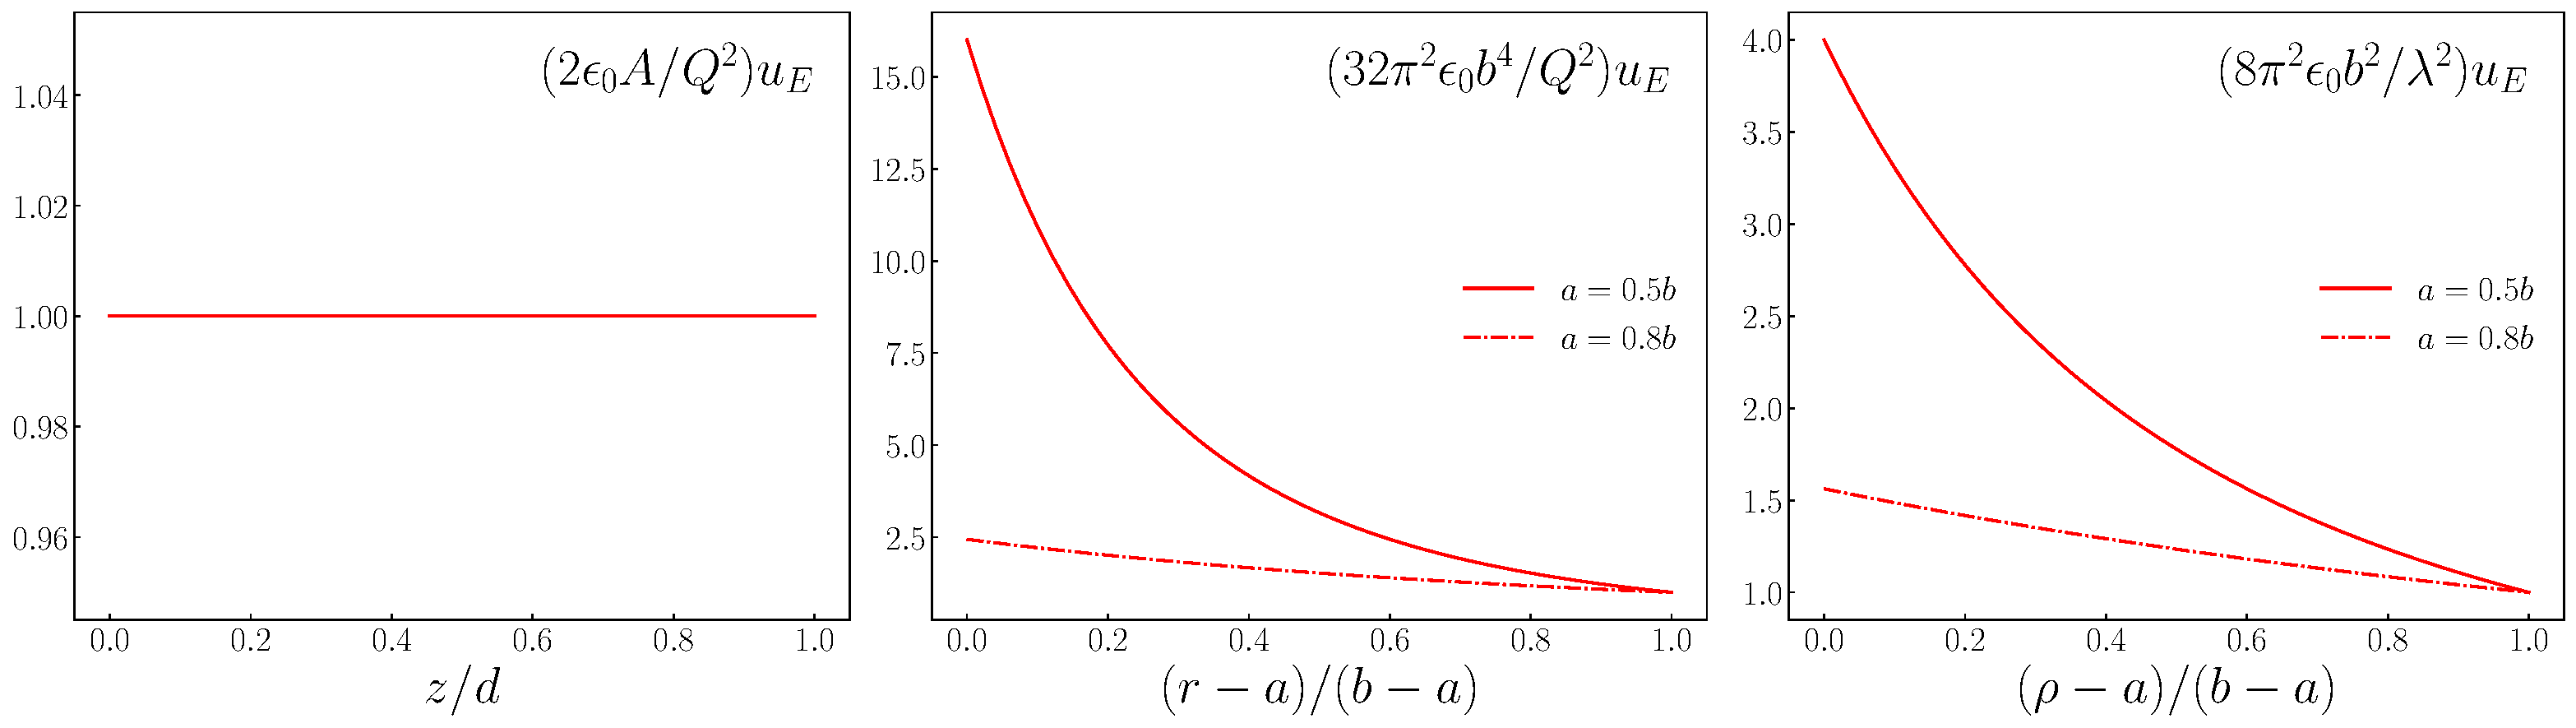
\includegraphics[width=\textwidth]{prob5.pdf}
    \caption{Plots of the energy density (normalized to be dimensionless) for \textbf{(Left)} a parallel plate capacitor (constant), \textbf{(Center)} spherical shell capacitor ($\sim r^{-4}$), and \textbf{(Right)} cylindrical shell capacitor ($\sim \rho^{-2}$).}
    \label{fig:prob5}
\end{figure}

}

\newpage

\prob{6}{

    Calculate the attractive force between conductors in the parallel plate capacitor (Problem 4(a)) for \\[3pt]

(a) fixed charges on each conductor; \\[3pt]

(b) fixed potential difference between conductors.

}

\sol{

(a) For the parallel plate capacitor, the work required to separate the plates by $\dd{x}$ 
\begin{eqnarray}
    \dd{W} = F \dd{x} = -\dd{U}
.\end{eqnarray}
In this instance, we do not care too much about the sign since the plates are oppositely charged and therefore attract each other overall.

The total energy stored in the plates when separated by a distance $x$ is
\begin{eqnarray}
   U = \frac{Q^2 x}{2 A \epsilon_0}
,\end{eqnarray}
implying that the force at a distance $d$ between the plates is attractive with magnitude
\begin{eqnarray}
    \label{eq:F-constQ}
    \eqbox{ F = \Big| \Big( \pdv{U}{x} \Big)_{Q} \Big| = \frac{Q^2}{2 A \epsilon_0} }
.\end{eqnarray}

(b) By a similar line of reasoning, holding the potential difference constant as the plates are separated, we find the force between the plates is attractive again with magnitude
\begin{eqnarray}
    \label{eq:F-constV}
    \eqbox{ F = \Big| \Big( \pdv{U}{x} \Big)_{V} \Big| = \frac{A \epsilon_0 V^2}{2d^2}}
.\end{eqnarray}
A simple sanity check is that if the end state is the same for both procedures, then the forces on the plates should be the same.
Using the relation $V = Qd/A\epsilon_0$, we find that \eref{F-constV} yields \eref{F-constQ} as desired.

}


\end{document}
